\documentclass{ximera}  
\title{Flowcharts with Operators}  
\begin{document}  
\begin{abstract}  
We introduce some mathematical notation to help us create algorithms to solve mathematical problems. 
\end{abstract}  
\maketitle

\section{Operators}
Many of the problems we will encounter in this course will require that we perform some iterative process or compute some quantity. For example:

\begin{enumerate}
	\item Compute the sum $1+2+3+\cdots+16$.
	\item Count the number of divisors of $100$.
	\item Determine the value of your account after 10 years if you invest \$1000 into a savings account that offers a $4$\% interest rate compounded monthly.
	\item Sort the list of numbers 1, 5, 6, 2, 3, 8, 4 in ascending order.
\end{enumerate}

When creating algorithms to solve these types of problems, we will often need to compare quantities or keep track of (and update) certain values. To help us with this we introduce some important notation and conventions. (Note that this list is not exhaustive.)

\begin{itemize}
	\item Assignment (\verb|:=|) - This operator assigns the value of whatever is on the right to whatever is on the left. For example, \verb|x:=2| assigns the value \verb|2| to the variable \verb|x|. Note that \verb|x:=y| and \verb|y:=x| are not the same. Also, a statement like \verb|x:=x+1| increments the value of \verb|x| by 1.
	\item Comparison (\verb|=|,\verb|<|,\verb|>|,\verb|<=|,\verb|>=|) - These operators are used for comparisons. They give back a truth value to help determine which route to take in a conditional operation/decision. For example, \verb|x>0| will be true if the value of \verb|x| is larger than 0 and false otherwise.
		\item Arithmetic (\verb|+|,\verb|-|,\verb|*|,\verb|**|,\verb|/|,\verb|%|) - These symbols simply perform the particular operations that we are used to. Note that \verb|**| represents exponentiation and \verb|%| is modular division (it returns the remainder after long division). For example, \verb|2**3| equals 8 and \verb|7%3| is equal to 1.
\end{itemize}

The assignment and equality comparison operators given above are not given as they are used in Python or other programming languages. The notation above is used in pseudocode, which is a generic, programming language independent way to express algorithms. In later sections we will give examples of how to use these operators in Python. 

Here is an example of an algorithm that determines if a number $n$ is divisible by 3. If the number is divisible by 3, the algorithm outputs a 1. Otherwise, the algorithm outputs a 0.

\begin{center}
	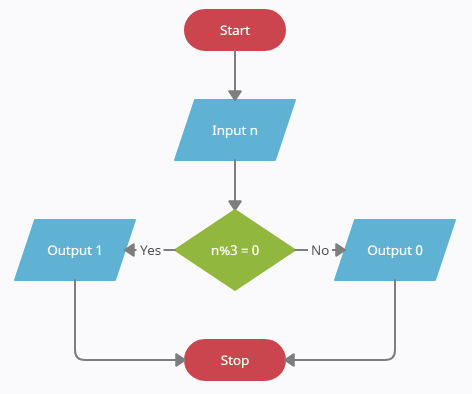
\includegraphics{divby3.png}
\end{center}

Here is an example of an algorithm that solves the linear equation $Ax+B=C$ for $x$ if $A$, $B$, and $C$ are real numbers with $A\neq 0$. (Why do we need to assume that $A\neq 0$?)

\begin{center}
	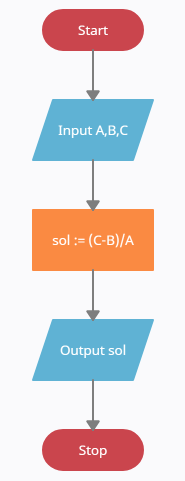
\includegraphics{solvelinear.png}
\end{center}

The following two examples illustrate a concept we will see over and over again. These flowcharts will have a loop showing that a certain step may be repeated multiple times until some condition is met.

Here is an example of an algorithm that finds the smallest integer greater than or equal to a real number $x\geq 0$.

\begin{center}
	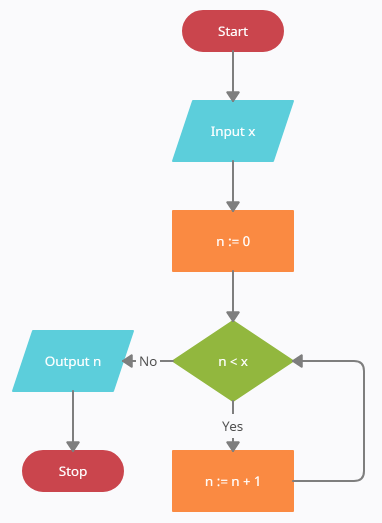
\includegraphics{ceil.png}
\end{center}

Here is an example of an algorithm that computes the sum $1+2+3+\cdots+n$ for any integer $n>0$.

\begin{center}
	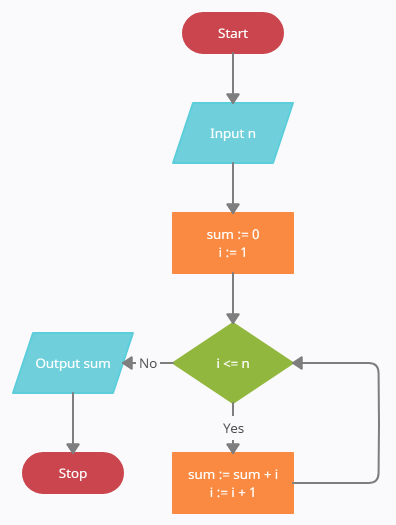
\includegraphics{gausssum.png}
\end{center}

\section{Problems}

\begin{question}
	A divisor $m$ of $n$ is any integer $m$ such that there is no remainder when dividing $n$ by $m$. Create an algorithm that counts the number of divisors of $n$ for any integer $n>0$. 
	\begin{hint}
	You may need two decisions to solve this problem. Note that the second hint for this problem is the solution.
	\end{hint}

	\begin{hint}
	\begin{center}
		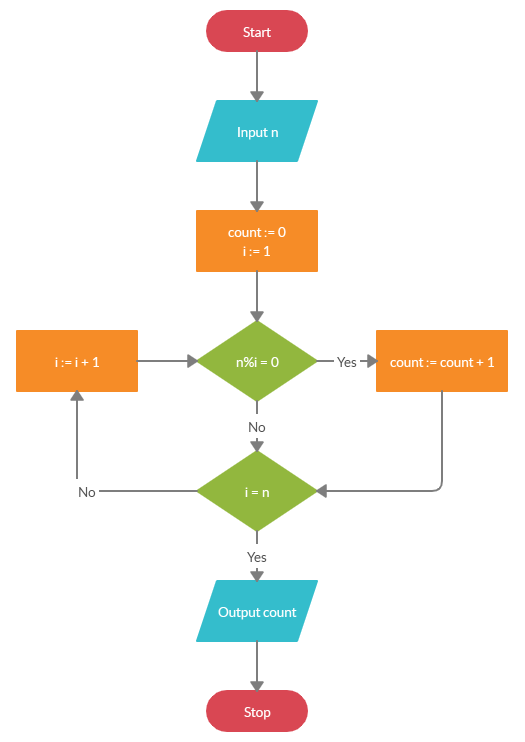
\includegraphics{divcount.png}
	\end{center}
	\end{hint}
\end{question}

\begin{question}
	Create an algorithm that determines if a positive integer is a prime number. Prime numbers are integers greater than 1 that have exactly two distinct divisors.
	\begin{hint}
		You should be able to modify the divisor count algorithm above. Note that the second hit for this problem is the solution.
	\end{hint}
	\begin{hint}
	\begin{center}
		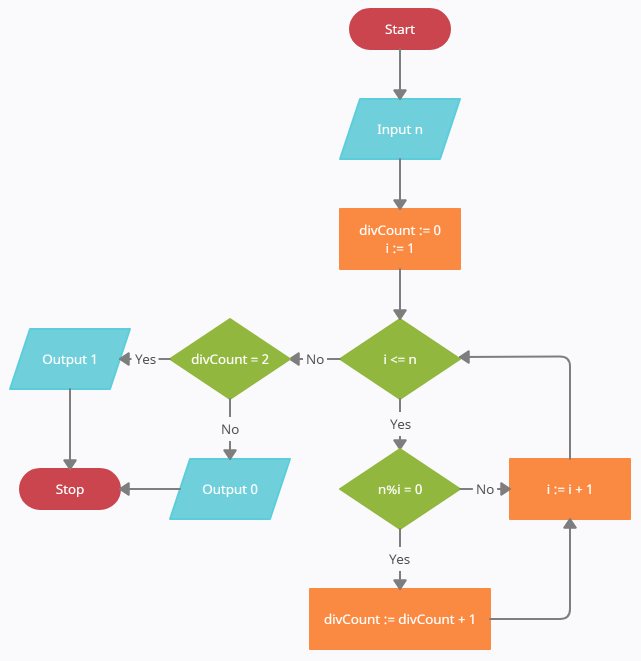
\includegraphics{primes.png}
	\end{center}
	\end{hint}
\end{question}

\end{document}
